% !TeX root = main.tex
\cleardoublepage
\fancyfoot[L]{\small \RomanNumeralCaps{2}}

\section{Flow of an incompressible fluid; Bernoulli's law}
\label{sec:bernoulli}

    This is a problem of ideal-fluid hydrodynamics, and it rests on three simplifications:

    \begin{itemize}
        \item the fluid is incompressible, that is, it does not change its volume under pressure, which for liquids is usually a very good approximation
        \item friction arising from the viscosity of the liquid is negligible
        \item the flow of the liquid is steady and irrotational: at any fixed point in the pipe the velocity, density and so on do not change with time, and the fluid elements are carried along without spinning about themselves
    \end{itemize}

    Applying the principle of conservation of energy to the flow problem, one obtains Bernoulli's law, which is usually written as:

    \begin{empheq}[box=\fbox]{equation}\label{eq:bernoulli}
        \frac{v^2}{2} + gh + \frac{p}{\rho} = \const
    \end{empheq}
    \keyeqentry{Bernoulli's law}

    where we have, in turn, the kinetic energy, the potential energy and the energy due to pressure, each per unit mass of fluid. The constant keeps the same value all along a \emph{streamline}, meaning the path traced out by a small parcel of fluid as it is carried by the flow, and because the flow was assumed irrotational the same constant in fact serves the whole flow. The relation permits the description of flow through a pipe that changes its cross-section or its height, and it explains the so-called hydrodynamic paradox. Where a pipe narrows, incompressibility forces the liquid to flow faster, since the same volume must pass each second through a smaller area, so by \cref{eq:bernoulli} the larger $\nicefrac{v^2}{2}$ must be offset by a smaller pressure $p$. The counter-intuitive result is that the pressure is \emph{lower} where the pipe is narrow and the flow is fast.

\section{Maxwell's equations, the scalar and vector potentials of the electromagnetic field, the equations of the electromagnetic field in vacuum and in media}
\label{sec:maxwell}

    \subsection{Maxwell's equations --- general form}

        \begin{empheq}[box=\fbox]{equation}\label{eq:maxwell-general}
            \begin{alignedat}{2}
                \text{Gauss's law for } \vec{E}                                 & : \quad & \nabla \cdot \vec{E}  & = \frac{\rho_{\text{f}} + \rho_{\text{b}}}{\varepsilon_{0}}\\
                \text{Gauss's law for } \vec{B}                                 & : \quad & \nabla \cdot \vec{B}  & = 0\\
                \text{Faraday's law}                                            & : \quad & \nabla \times \vec{E} & = -\frac{\partial \vec{B}}{\partial t}\\
                \text{Ampère--Maxwell law}                                      & : \quad & \nabla \times \vec{B} & = \mu_{0}\left(\vec{J_{\text{f}}} + \vec{J_{\text{b}}} + \varepsilon_{0}\frac{\partial\vec{E}}{\partial t}\right),
            \end{alignedat}
        \end{empheq}
        \keyeqentry{Maxwell's equations---general form}

        where $\rho$ is a charge density, $\vec{J}$ a current density, $\vec{E}$ the electric field and $\vec{B}$ the \emph{magnetic flux density} (or sometimes \emph{magnetic induction}). Charges and currents are of two kinds. \emph{Free} ones ($\rho_{\text{f}}$, $\vec{J}_{\text{f}}$) are the ones we put there and control, such as the conduction electrons in a wire or the charge deposited on a plate. \emph{Bound} ones ($\rho_{\text{b}}$, $\vec{J}_{\text{b}}$) are locked inside the atoms of a material and can only shift or circulate slightly without leaving them, and it is the applied field itself that induces them. 
        
        The fields make no such distinction---only the total charge and current act as sources---but it is worth making, because the bound part is a response of the material and can be absorbed into redefined fields (\cref{sec:maxwell-matter}).

        The nabla operator $\nabla$ (\cref{eq:nabla}) can be used to mean different operations, giving:

        \begin{equation*}
            \begin{aligned}
                \nabla \cdot \vec{A} &\text{ --- divergence of a vector field}\\
                \nabla \times \vec{A} &\text{ --- curl of a vector field}\\
                \nabla f &\text{ --- gradient of a scalar field}
            \end{aligned}
        \end{equation*}

        Divergence measures how strongly a given point acts as a source or a sink of a vector field, curl measures the circulation of the field around a point, and the gradient points in the direction in which a scalar field increases fastest. Two integral theorems turn these statements about single points into statements about whole regions. The \emph{divergence theorem} says that the divergence added up over a volume equals the flux out through the surface enclosing it,\todoper{check kcl math notes}

        \begin{equation}\label{eq:divergence-theorem}
            \int_{V}\nabla\cdot\vec{A}\,dV = \oint_{\partial V}\vec{A}\cdot d\vec{S},
        \end{equation}

        and \emph{Stokes' theorem} says that the curl added up over a surface equals the circulation of the field around the loop bounding it,

        \begin{equation}\label{eq:stokes-theorem}
            \int_{S}\left(\nabla\times\vec{A}\right)\cdot d\vec{S} = \oint_{\partial S}\vec{A}\cdot d\vec{l} .
        \end{equation}

        Applied to \cref{eq:maxwell-general} they give each equation its plain reading:

        \begin{itemize}
            \item \textbf{Gauss's law for $\vec{E}$.} The electric flux out through any closed surface is fixed by the charge enclosed and by nothing else. Field lines start on positive charge and end on negative charge.
            \item \textbf{Gauss's law for $\vec{B}$.} The magnetic flux out through any closed surface is always zero, so magnetic field lines have no ends and close on themselves. There is no magnetic charge for them to start from---no magnetic monopole has ever been observed.
            \item \textbf{Faraday's law.} Time-varying magnetic field gives rise to the rotational electric field. The minus sign is Lenz's law, which says that the induced current flows in such a direction as to oppose the change that produced it.
            \item \textbf{Ampère--Maxwell law.} A current due to bound/free charges \emph{or} a time-varying electric field give rise to rotational magnetic field.
        \end{itemize}

        Fields act on charges through the Lorentz force. Essentailly all electromagnetism can be derived from it:

        \begin{equation}\label{eq:lorentz-force}
            \vec{F}=q\,(\vec{E}+\vec{v}\times\vec{B})
        \end{equation}

    \subsection{Maxwell's equations in vacuum}

        In vacuum there are no charges or currents at all, free or bound, so $\rho = 0$ and $\vec{J} = 0$, and Maxwell's equations reduce to their source-free form that only describe the action of the fields:

        \begin{equation}\label{eq:maxwell-vacuum}
            \begin{aligned}
                \nabla \cdot \vec{E}  & = 0\\
                \nabla \cdot \vec{B}  & = 0\\
                \nabla \times \vec{E} & = -\frac{\partial \vec{B}}{\partial t}\\
                \nabla \times \vec{B} & = \mu_{0}\varepsilon_{0}\frac{\partial\vec{E}}{\partial t}
            \end{aligned}
        \end{equation}

    \subsection{Maxwell's equations in matter}
    \label{sec:maxwell-matter}

        An electric field pulls the positive and negative charge of each atom or molecule slightly apart, giving it an electric dipole moment $\vec{p} = q\vec{d}$, where $\vec{d}$ points from the negative charge to the positive one. Averaged per unit volume these moments give the polarisation vector $\vec{P}$ (\cref{sec:electric-field}), which in a linear dielectric is proportional to the field,

        \begin{equation}\label{eq:polarisation-vector}
            \vec{P}=\chi \varepsilon_0\vec{E},
        \end{equation}

        where $\chi$ --- electric susceptibility of a material. Polarisation moves bound charge only, and

        \begin{equation}\label{eq:bound-charge}
            \nabla\cdot\vec{P}=-\rho_{\text{b}}.
        \end{equation}

        Since $\vec{P}$ points from the negative end of each dipole to the positive end, a region out of which $\vec{P}$ spreads (positive divergence) is one from which positive bound charge has been carried away, so what remains there is negative. In other words, the electric field that is caused by $\vec{P}$ points roughly in the opposite direction to $\vec{P}$.

        From Gauss's law for the electric field, we then have

        \begin{equation*}
            \begin{aligned}
                \nabla\cdot(\varepsilon_0\vec{E})          &= \rho_{\text{f}} + \rho_{\text{b}} \\
                \nabla\cdot(\varepsilon_0\vec{E}+\vec{P})  &= \rho_{\text{f}}, \\
                \nabla\cdot\vec{D} &= \rho_{\text{f}},
            \end{aligned}
        \end{equation*}

        where $\vec{D}$ --- the electric displacement field,

        \begin{empheq}[box=\fbox]{equation}\label{eq:D-def}
            \vec{D} \equiv \varepsilon_{0}\vec{E} + \vec{P} .
        \end{empheq}
        \keyeqentry{Electric displacement field}

        Adding $\vec{P}$ cancels the bound charge contributions (\cref{eq:bound-charge}), so $\vec{D}$ is the field whose sources are the free charges alone---the ones we control. $\vec{P}$ points in the opposite direction to the field it is producing, so it subtracts from $\vec{E}$.

        Matter responds magnetically as well. Every atom carries a small circulating current (\cref{eq:orbital-angular-momentum,subsec:quantum-precession}) and so a magnetic dipole moment, which for a simplest model of a wire-carrying loop is defined as $\vec{\mu} = I\vec{A}$, where $I$ is the current and $\vec{A}$ is the area vector of the loop. The average moment per unit volume is the \emph{magnetisation} $\vec{M}$. Inside a uniformly magnetised body, neighbouring loops run in opposite directions where they meet and cancel, so a net current survives only at the surface, or anywhere $\vec{M}$ varies from place to place. Added up, what is left is $\nabla\times\vec{M}$. A polarisation that changes in time is on top of that a genuine motion of bound charge, hence a current $\nicefrac{\partial\vec{P}}{\partial t}$. The two together make the bound current

        \begin{equation*}
            \vec{J}_{\text{b}} = \nabla\times\vec{M} + \frac{\partial\vec{P}}{\partial t}.
        \end{equation*}

        From the Ampère--Maxwell law, we then have

        \begin{equation*}
            \begin{aligned}
                \nabla\times\vec{B}                                     & = \mu_{0}\left(\vec{J_{\text{f}}} + \vec{J_{\text{b}}} + \varepsilon_{0}\frac{\partial\vec{E}}{\partial t}\right) \\
                                                                        & = \mu_{0}\left(\vec{J_{\text{f}}} + \nabla\times\vec{M} + \frac{\partial\vec{P}}{\partial t} + \varepsilon_{0}\frac{\partial\vec{E}}{\partial t}\right) \\
                \nabla\times\vec{H}  & = \vec{J_{\text{f}}} + \frac{\partial \vec{D}}{\partial t},
            \end{aligned}
        \end{equation*}

        where $\vec{H}$ --- the \emph{magnetic field} (or \emph{magnetic field strength/intensity}),

        \begin{empheq}[box=\fbox]{equation}\label{eq:H-def}
            \vec{H} \equiv \frac{\vec{B}}{\mu_{0}} - \vec{M} .
        \end{empheq}
        \keyeqentry{Magetic field strength}

        The minus here does the same job as the plus in \cref{eq:D-def}. Moving $\nabla\times\vec{M}$ to the left-hand side of the equation above is what subtracts $\vec{M}$, and it removes the bound magnetisation current from the curl, leaving $\vec{H}$ sourced by free currents alone. Both $\vec{D}$ and $\vec{H}$ are therefore devices for hiding the material's own response inside a redefined field, so that only the sources we control appear explicitly.

        \needspace{4\baselineskip}
        Maxwell's equation in matter may then finally be rewritten as:

        \begin{empheq}[box=\fbox]{equation}\label{eq:maxwell-media}
            \begin{aligned}
                \nabla \cdot \vec{D} &= \rho_{\text{f}}\\
                \nabla \cdot \vec{B} &= 0\\
                \nabla\times\vec{E} &= -\frac{\partial \vec{B}}{\partial t}\\
                \nabla\times\vec{H} &= \vec{J}_{\text{f}} + \frac{\partial\vec{D}}{\partial t}
            \end{aligned}
        \end{empheq}
        \keyeqentry{Maxwell's equations---in matter}

    \subsection{The scalar and vector potentials}\label{sec:em-potentitals}

        Two of Maxwell's equations carry no sources at all, and they can be satisfied identically---made true by construction---once the fields are written in terms of potentials.

        Since $\nabla\cdot\vec{B} = 0$ everywhere, and since \emph{the divergence of any curl vanishes automatically}, $\vec{B}$ may always be written as the curl of some vector field,

        \begin{empheq}[box=\fbox]{equation}\label{eq:vector-potential}
            \vec{B} = \nabla\times\vec{A},
        \end{empheq}
        \keyeqentry{Magnetic vector potential}

        called the \emph{magnetic vector potential}. Substituting this into Faraday's law gives $\nabla\times\left(\vec{E} + \nicefrac{\partial\vec{A}}{\partial t}\right) = 0$, and \emph{a field whose curl vanishes is the gradient of something}, so

        \begin{empheq}[box=\fbox]{equation}\label{eq:scalar-potential}
            \vec{E} = -\nabla\varphi - \frac{\partial\vec{A}}{\partial t},
        \end{empheq}
        \keyeqentry{Electric scalar potential and electric field}

        where $\varphi$ is the \emph{electric scalar potential}. In electrostatics the second term is absent and $\varphi$ is the familiar potential whose difference between two points is a voltage and can express avarage electric field as ($E=\nicefrac{\Delta V}{\Delta x}$).

       The gain is economy. The two source-free equations are now satisfied automatically and only the two with sources remain to be solved, and the six components of $\vec{E}$ and $\vec{B}$ are traded for four, $\varphi$ and $\vec{A}$. The potentials are not unique: adding $\nabla f$ to $\vec{A}$ while subtracting $\nicefrac{\partial f}{\partial t}$ from $\varphi$ leaves both fields exactly as they were, for any scalar function $f(\vec{r},t)$. Such a substitution is a \emph{gauge transformation}, and the insensitivity of the fields to it is \emph{gauge invariance}. The freedom is used to impose whichever extra condition makes a given problem easiest. The potentials are also what enter the Lagrangian of a charged particle, and hence its quantum mechanics, so they are more than a calculational convenience. In relativistic electrodynamics they combine into a single four-vector (\cref{sec:inertial-frames}),
        \begin{equation*}
            A^{\mu} =
            \begin{bmatrix}
                \nicefrac{\varphi}{c} \\ \vec{A}
            \end{bmatrix},
        \end{equation*}

        whereas $\vec{E}$ and $\vec{B}$ need a rank-2 tensor to hold their six components. The potentials are the more natural relativistic objects as well as the more economical ones.
        
\section{The electric field in media; dielectric polarisation, conduction, mobility of the charge carriers}
\label{sec:electric-field}

    \subsection{Polarisation}

        Dielectric polarisation is the formation of electric dipoles, or the alignment of ones already present, under an applied electric field. The dipoles set up a field of their own inside the material which partly cancels the applied field, so the field inside a dielectric is always weaker than the field applied to it. Averaged per unit volume the dipole moments give the polarisation vector $\vec{P}$, whose linear form and role in Maxwell's equations are set out in \cref{sec:maxwell-matter}.

        The response is only approximately linear. In general $\vec{P}$ is expanded in powers of the field, written here for one direction,

        \begin{equation}\label{eq:nonlinear-polarisation}
            P = \varepsilon_{0}\left(\chi^{(1)}E + \chi^{(2)}E^{2} + \chi^{(3)}E^{3} + \cdots\right),
        \end{equation}

        where $\chi^{(1)} \equiv \chi$ --- the linear electric susceptibility of \cref{eq:polarisation-vector}. The higher coefficients are so small that the extra terms matter only in intense laser fields, where they are the whole of \emph{nonlinear optics}: $\chi^{(2)}$ lets a crystal double the frequency of the light passing through it (second-harmonic generation), and $\chi^{(3)}$ makes the refractive index depend on the intensity in the optical range. Strictly each $\chi^{(k)}$ is a tensor, since $\vec{P}$ need not point along $\vec{E}$ in an anisotropic crystal, which is the origin of birefringence.

        Keeping the linear term alone and substituting it into the definition of the displacement field (\cref{eq:D-def}) gives

        \begin{equation}\label{eq:permittivity}
            \vec{D} = \varepsilon_{0}\vec{E} + \vec{P} = \varepsilon_{0}\left(1+\chi\right)\vec{E} \equiv \varepsilon_{0}\varepsilon_{\text{r}}\vec{E},
        \end{equation}

        where $\varepsilon_{\text{r}} \equiv 1+\chi$ --- relative permittivity (dielectric constant) of the material, which fixes the refractive index (\cref{eq:refractive-index}). It is $1$ in vacuum and a few for ordinary glasses and plastics, but in general it is complex and frequency-dependent, its imaginary part recording absorption, and in a metal below the plasma frequency it is negative---which is what governs the behaviour of EM waves in media (\cref{sec:em-waves}). The three mechanisms below add up to it (\cref{eq:polarisability-sum}), and each stops contributing at a different frequency.

        Underneath $\chi$ there is a microscopic picture. Each atom or molecule acquires the dipole moment $\vec{p} = q\vec{d}$ (\cref{sec:maxwell-matter}), and in a weak field it is proportional to the field acting on it,

        \begin{empheq}[box=\fbox]{equation}\label{eq:polarisability}
            \vec{p} = \alpha\vec{E},
        \end{empheq}
        \keyeqentry{Polarisability}

        where $\alpha$ --- the \emph{polarisability}, a measure of how easily that particular atom or molecule is deformed or turned. With $N$ such units per unit volume the polarisation is their sum, $\vec{P} = N\vec{p}$, and comparing it with \cref{eq:polarisation-vector} gives $\chi = \nicefrac{N\alpha}{\varepsilon_{0}}$. Strictly the $\vec{E}$ of \cref{eq:polarisability} is the field at the site of the atom rather than the macroscopic average field, and correcting for the difference turns it into the Clausius--Mossotti formula.
        
        The three mechanisms below are not alternatives. Every material has electrons, so the electronic contribution is always present, and a material whose structure permits the others shows them at the same time. Their polarisabilities simply add,

        \begin{equation}\label{eq:polarisability-sum}
            \alpha = \alpha_{\text{e}} + \alpha_{\text{i}} + \alpha_{\text{or}},
        \end{equation}

        so that $\chi$, $\varepsilon_{\text{r}}$ and the weakened field inside the dielectric are always the net effect of whichever mechanisms are present. An ionic crystal such as NaCl has the first two, liquid water the first and the third.

        \paragraph{Electronic polarisation}

            Electronic polarisation is the displacement of an atom's negatively charged electron cloud with respect to its positive nucleus, inducing a moment governed by $\alpha_{\text{e}}$. Its polarisability grows roughly with the volume of the atom, since a larger and more loosely bound cloud is easier to pull aside. Only the light electrons have to move, so it is much the fastest of the three and still follows the field at optical and ultraviolet frequencies---it is what supplies the refractive index of ordinary glass.

        \paragraph{Ionic polarisation}

            Ionic polarisation occurs only in materials with ionic bonds. It is the displacement of the ions of the crystal lattice, those of one sign one way and those of the other sign the other way, with a polarisability $\alpha_{\text{i}}$ of the same induced kind as the electronic one. Whole atoms bound in a lattice must move, so it is far slower than the electronic mechanism and dies out above the infrared.

        \begin{minipage}{1\textwidth}
            \paragraph{Orientational polarisation}
            \begin{wrapfigure}{L}{0.2\textwidth}
                    \centering
                    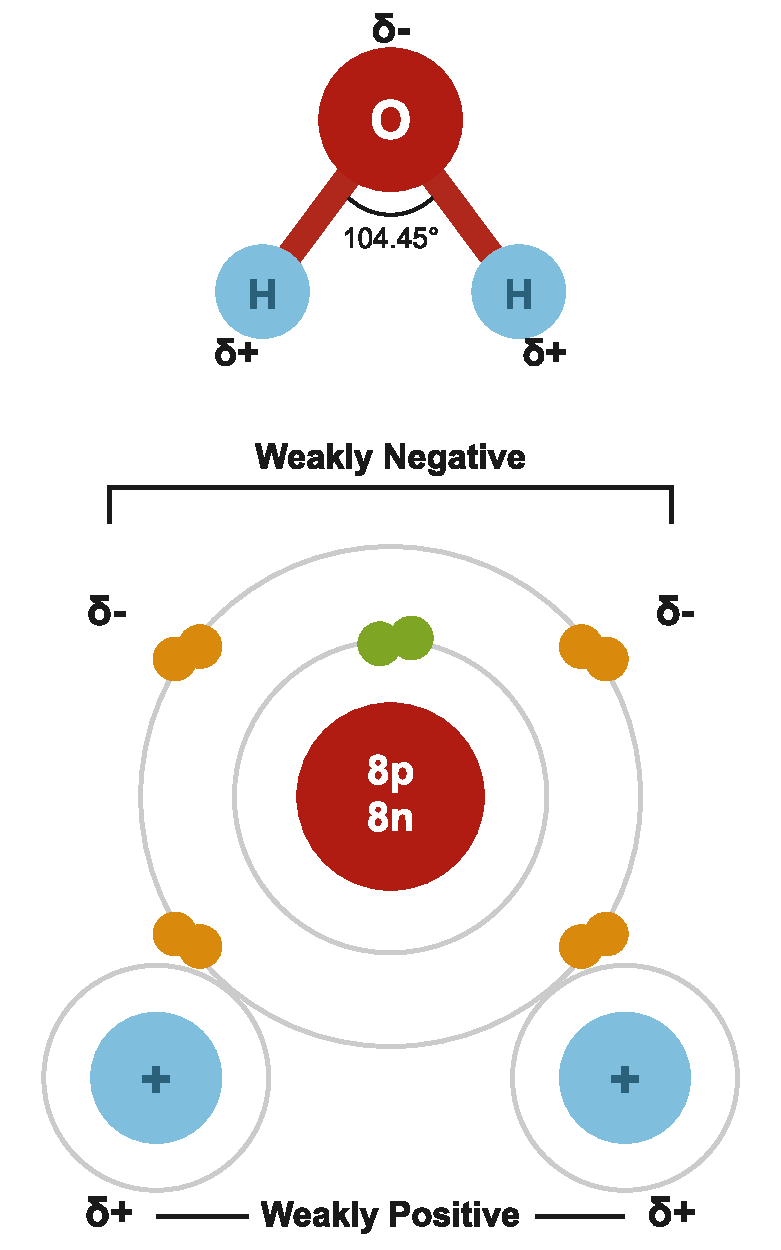
\includegraphics[width=0.18\textwidth]{graphics/water_molecule.pdf}
                    \caption{Water molecule.}
                    \label{fig:water-molecule}
                \end{wrapfigure}

                Orientational polarisation, also called dipolar polarisation, occurs only in polar dielectrics, that is, in materials whose molecules carry a permanent dipole moment $p_{0}$ of their own. The field exerts an ordering torque on them while thermal motion destroys the ordering, so what survives is a slight statistical bias in their directions. Nothing is deformed here and no single moment changes size, so the polarisability is an effective one produced by that averaging,

                \begin{equation}\label{eq:orientational-polarisability}
                    \alpha_{\text{or}} = \frac{p_{0}^{2}}{3\kB T},
                \end{equation}

                valid while the ordering energy $p_{0}E$ stays small against $\kB T$. This is the only contribution that depends on temperature, and it falls as the material is heated. Whole molecules must reorient, so it is the slowest mechanism of all and stops following the field somewhere in the microwave range---which is exactly what a \emph{microwave oven} exploits in water (\cref{fig:water-molecule}).
        \end{minipage}

    \subsection{Conductivity and mobility}

        Conduction is the flow of electric charge through a material under an applied field. The carriers do not accelerate freely, because they are scattered by lattice vibrations and by defects, so in a steady field they settle at an average \emph{drift velocity} $v_{\text{d}}$ proportional to the field. The constant of proportionality is the \emph{mobility},

        \begin{empheq}[box=\fbox]{equation}\label{eq:mobility}
            \mu_{\text{c}} \equiv \frac{v_{\text{d}}}{E},
        \end{empheq}
        \keyeqentry{Mobility}

        which measures how easily a carrier is pushed through a particular material. The current density is then $J = qnv_{\text{d}} = \sigma E$, the local form of Ohm's law, with the \emph{conductivity}

        \begin{empheq}[box=\fbox]{equation}\label{eq:conductivity}
            \sigma = qn\mu_{\text{c}},
        \end{empheq}
        \keyeqentry{Conductivity}

        where $q$ is the charge of one carrier and $n$ their concentration. Only two things can therefore change a conductivity: \emph{how many carriers there are, and how freely each moves}. Temperature acts on both factors in \cref{eq:conductivity}, $n$ and $\mu_{\text{c}}$, and which one wins distinguishes the two standard cases.

        \begin{table}[H]
            \centering
            \begin{minipage}[t]{0.41\textwidth}\vspace{0pt}
                \centering
                \small
                \renewcommand{\arraystretch}{1.25}
                \begin{tabularx}{\linewidth}{@{}lLL@{}}
                    \hline
                    \textbf{kind} & \textbf{carrier} & \textbf{sign} \\
                    \hline
                    electronic & electrons in the conduction band & negative \\
                    hole & vacancies in an otherwise full valence band & positive \\
                    ionic & whole ions & either \\
                    \hline
                \end{tabularx}
                \captionof{table}{The three most common kinds of conduction, classified by carrier.}
                \label{tab:conduction-kinds}
            \end{minipage}%
            \hfill
            \begin{minipage}[t]{0.53\textwidth}\vspace{0pt}
                \centering
                \small
                \renewcommand{\arraystretch}{1.25}
                \begin{tabularx}{\linewidth}{@{}lLLL@{}}
                    \hline
                    \textbf{material} & \textbf{$n(T)$} & \textbf{$\mu_{\text{c}}(T)$} & \textbf{net $\sigma(T)$} \\
                    \hline
                    metal & fixed & falls (more scattering) & falls \\
                    semiconductor & rises steeply (thermal excitation across the gap) & falls, but this loses out & rises \\
                    \hline
                \end{tabularx}
                \captionof{table}{Temperature dependence of conductivity in a metal versus a semiconductor.}
                \label{tab:conduction-temperature}
            \end{minipage}
        \end{table}

        In a metal $n$ is fixed, while more lattice vibrations mean more scattering and a smaller $\mu_{\text{c}}$, so the conductivity falls as the material is heated. In a semiconductor $n$ rises steeply with temperature, because carriers must first be excited across the band gap, and that easily outweighs the loss of mobility, so the conductivity rises instead. The conduction band, the valence band and the gap between them are set out in \cref{sec:bands}.

\section{The magnetic field in media; classification of magnetic media, microscopic description of interactions between the magnetic moments of components of the medium (atoms, ions, molecules)}
\label{sec:magnetic-field}

    On the microscopic scale every medium has magnetic properties, on account of the spin of its constituent particles and of the motion of the electrons about the nuclei. On the macroscopic scale magnetic behaviour is far less common, because these moments are not ordered over long distances and largely cancel one another. Long-range order can be imposed by an external magnetic field, just as polarisation is imposed by an electric one (\cref{sec:electric-field}).

    The bookkeeping is also the same. The average magnetic dipole moment per unit volume is the magnetisation $\vec{M}$, and it is hidden inside the redefined field $\vec{H} \equiv \nicefrac{\vec{B}}{\mu_{0}} - \vec{M}$ (\cref{eq:H-def}), which is sourced by the free currents we control and by nothing else (\cref{sec:maxwell-matter}). Taking the response to be linear in $\vec{H}$,

    \begin{equation}\label{eq:magnetic-susceptibility}
        \vec{M} = \chi_{m}\vec{H} \quad \Longrightarrow \quad \vec{B} = \mu_{0}\left(1+\chi_{m}\right)\vec{H} \equiv \mu_{0}\mu_{\text{r}}\vec{H},
    \end{equation}

    where $\chi_{m}$ --- magnetic susceptibility, and $\mu_{\text{r}} \equiv 1+\chi_{m}$ --- relative permeability, the exact counterpart of $\varepsilon_{\text{r}} = 1+\chi$ (\cref{eq:permittivity}). A difference is worth noting: $\chi$ is positive for ordinary dielectrics, whereas $\chi_{m}$ may have either sign, and its sign is what classifies the material. For most media $|\chi_{m}| \sim 10^{-5}$, so magnetically they are almost vacuum ($\mu_{\text{r}} \simeq 1$), while in a ferromagnet $\chi_{m}$ reaches $10^{3}$ or more and the linear relation fails altogether.
    
    Interactions with a magnetic field are also more subtle than with an electric one: by the Bohr--van Leeuwen theorem a purely classical system in equilibrium has zero mean magnetisation, so every magnetic effect below is a quantum one. Three kinds of medium are usually distinguished.

    Three kinds of medium are usually distinguished, and the first division between them is whether the material has any magnetism of its own. Paramagnets and diamagnets do not: each merely responds while an external field is applied, with a magnetisation proportional to it and vanishing the moment it is removed, and the two differ only in the sign of that response. Ferromagnets, antiferromagnets and ferrimagnets do, because their moments order one another rather than waiting to be ordered by the field, so they keep a magnetisation after the field is switched off.\todo{check}

    \subsection{Paramagnets}

        The most common group. They have \emph{positive susceptibility}, so the induced \emph{magnetisation points along the applied field}. It comes from \emph{unpaired electrons}, whose magnetic moments turn to line up with an external field. Common paramagnets are aluminium, platinum and oxygen. Two standard models:

        \begin{itemize}
            \item Curie paramagnetism --- a set of independent atomic moments that do not interact with one another. Balancing their alignment against the randomising effect of heat gives Curie's law for the susceptibility,
            \begin{equation*}
                \chi_m = \frac{C}{T},
            \end{equation*}
            where $T$ is the absolute temperature and $C$ (the Curie constant) is fixed by the size and number of the atomic moments. The susceptibility falls as the temperature rises because thermal agitation fights the alignment.
            \item Pauli paramagnetism---in a metal the conduction electrons (as in an ordinary metal such as sodium) are treated as a \emph{Fermi gas}: a gas of electrons that barely interact, but which (because no two electrons may share the same quantum state, \cref{eq:identical}) fill the available energy levels from the bottom up to a top level called the \emph{Fermi level}. Confining the electrons to the metal leaves them only a discrete ladder of allowed energies, so tightly spaced as to look continuous, and each rung holds one electron. Stacking them from the bottom up is forced: an electron deep in the pile cannot change its state at all, because every neighbouring rung it might move to is already taken. Only near the top of the pile are there empty rungs within reach, and the energy of that topmost occupied rung is the Fermi level---a few electronvolts in a typical metal, which is some hundred times $\kB T$ at room temperature (\cref{sec:ensembles}). Only the few electrons near that top level are free to reorient in a field, so the resulting paramagnetism is weak and almost independent of temperature.
        \end{itemize}

    \subsection{Diamagnets}\label{sec:diamagnets}

        Diamagnetism is the appearance of a magnetisation \emph{opposite} to the applied field, i.e.\ a negative susceptibility. Every material has this response, but it is very weak, so we call a material a diamagnet only when it is the dominant effect. That happens when the atoms carry no permanent magnetic moment---all electron spins paired---so there is no paramagnetic contribution to mask it. Typical diamagnets are bismuth (the strongest ordinary one), copper, gold and water.

        A special case is that of \emph{superconductors}, which expel the magnetic field from their interior completely. The remaining diamagnets are described by:

        \begin{itemize}
            \item Langevin diamagnetism --- describes insulators (such as water and the inert gases), where the electrons are bound in atoms rather than free to conduct and all their spins are paired, so only the orbital moments are left. An applied field sets each orbit precessing, and that precession is a small current loop whose moment opposes the field (\cref{subsec:quantum-precession}).
            \item Landau diamagnetism --- treats the same Fermi gas of conduction electrons in a metal as Pauli paramagnetism, but now accounts for the field bending the electrons' orbital motion rather than flipping their spin. This orbital effect is diamagnetic.
        \end{itemize}

    \subsection{Ferromagnets, antiferromagnets and ferrimagnets}

        Another category, \emph{ferromagnets}, appears once we include the \emph{exchange interaction}---a quantum effect that makes neighbouring moments prefer to \emph{point the same way as each other}\todo{why?}, not just as the external field. Regions of aligned moments (magnetic domains) form, giving a strong susceptibility and \emph{remanent} magnetisation: magnetisation that survives after the external field is switched off, which is what makes a permanent magnet. The classic ferromagnets are iron, cobalt and nickel.

        Such materials are analysed with statistical-physics lattice models that differ in how freely each moment may point: the Ising model allows only up or down, the XY model allows any direction in a plane, and the Heisenberg model allows any direction in space (the most general).

        Closely related are \emph{antiferromagnets} and \emph{ferrimagnets}, in which neighbouring moments point in \emph{opposite} directions. In an antiferromagnet the opposing moments are equal and cancel, so there is almost no net magnetisation (manganese oxide and chromium are examples). In a ferrimagnet they are opposite but unequal, so the cancellation is only partial and a net magnetisation remains---macroscopically it behaves like a weaker ferromagnet (magnetite is the classic example).

\section{Electromagnetic waves as solutions of Maxwell's equations; polarisation, reflection and refraction of electromagnetic waves, the Doppler effect}
\label{sec:em-waves}

    \subsection{Electromagnetic waves as solutions of Maxwell's equations}

        An electromagnetic wave is a solution of the Maxwell equations. For the simplest case in vacuum (\cref{eq:maxwell-vacuum}), we do the following steps:
        \begin{enumerate}
            \item take the curl of Faraday's law;
            \item apply the vector identity: $\nabla\times(\nabla\times\vec{F}) = \nabla(\nabla\cdot\vec{F}) - \nabla^{2}\vec{F}$;
            \item substitute the first Maxwell equation;
            \item substitute the fourth Maxwell equation.
        \end{enumerate}

        So, the curl of Faraday's law $\nabla\times\vec{E} = -\nicefrac{\partial\vec{B}}{\partial t}$ is:

        \begin{equation*}
            \nabla\times\left(\nabla\times\vec{E}\right) = \nabla\times\left(- \frac{\partial\vec{B}}{\partial t}\right).
        \end{equation*}

        Then apply the identity:

        \begin{equation*}
            \begin{aligned}
                \mathrm{LHS} = \nabla\times\left(\nabla\times\vec{E}\right)                 &= \nabla\left(\nabla\cdot\vec{E}\right) - \nabla^{2}\vec{E} =  \nabla\left( 0 \right) - \nabla^{2}\vec{E} = - \Delta \vec{E}\\
                \mathrm{RHS} = \nabla\times\left(- \frac{\partial\vec{B}}{\partial t}\right) &= - \frac{\partial}{\partial t}\left(\nabla\times\vec{B}\right) = - \frac{\partial}{\partial t} \left( \mu_{0}\varepsilon_{0}\frac{\partial\vec{E}}{\partial t} \right) = - \mu_{0}\varepsilon_{0}\frac{\partial^{2}\vec{E}}{\partial t^{2}},
            \end{aligned}
        \end{equation*}

        and, for the LHS, we use the identity and the first Maxwell equation, and for the RHS, use the fourth Maxwell equation where

        \begin{equation*}
            \Delta \vec{F} = \nabla^{2} \vec{F} = \left( \frac{\partial^2}{\partial x^2} + \frac{\partial^2}{\partial y^2} + \frac{\partial^2}{\partial z^2} \right) \vec{F}
        \end{equation*}

        is the Laplacian operator.

        Equating both sides we obtain:

        \begin{equation}\label{eq:em-wave}
            \left(\Delta - \mu_{0}\varepsilon_{0}\frac{\partial^{2}}{\partial t^{2}}\right)\vec{E} = 0
        \end{equation}

        We proceed analogously with the fourth Maxwell equation and find the equation for $\vec{B}$.

        \begin{equation*}
            \left(\Delta - \mu_{0}\varepsilon_{0}\frac{\partial^{2}}{\partial t^{2}}\right)\vec{B} = 0
        \end{equation*}

        Both of these equations are standard forms of the wave equation, generally written as:

        \begin{equation*}
            \left(\Delta - \frac{1}{v^{2}}\frac{\partial^{2}}{\partial t^{2}}\right)\vec{F} = 0,
        \end{equation*}

        where $v$ is the propagation speed. From this it follows that the speed of propagation of an electromagnetic wave in vacuum is

        \begin{equation*}
            v = c = \frac{1}{\sqrt{\mu_{0}\varepsilon_{0}}}.
        \end{equation*}

        Performing the same derivation inside a homogeneous, non-magnetic medium \todo{where is the non-magnetic assumption made?} that carries no free charge, so that $\nabla\cdot\vec{E}=0$ and the magnetisation contributes nothing, the sources do not all cancel and we are left with

        \begin{equation*}
            \left(\Delta - \mu_{0}\varepsilon_{0}\frac{\partial^{2}}{\partial t^{2}}\right)\vec{E} = \underbrace{\mu_{0}\frac{\partial\vec{J}_{\text{f}}}{\partial t}}_{\substack{\text{important in} \\ \text{conductors}}} + \underbrace{\mu_{0}\frac{\partial^{2}\vec{P}}{\partial t^{2}}}_{\substack{\text{important in} \\ \text{insulators}}},
        \end{equation*}

        both terms being zero in vacuum. In a transparent insulator the first term is absent and linear polarisation response (\cref{eq:polarisation-vector}) collects the second one back into the left-hand side, replacing $\varepsilon_{0}$ by $\varepsilon_{0}(\chi + 1)=\varepsilon_{0}\varepsilon_{\text{r}}$\todo{correct?}. The wave equation is recovered with a smaller speed $v = \nicefrac{c}{n}$, where

        \begin{empheq}[box=\fbox]{equation}\label{eq:refractive-index}
            n \equiv \frac{c}{v} = \sqrt{\varepsilon_{\text{r}}\mu_{\text{r}}} \simeq \sqrt{\varepsilon_{\text{r}}}
        \end{empheq}
        \keyeqentry{Refractive index}

        is the \emph{refractive index}, the quantity that appears in Snell's law (\cref{eq:snell}), and the approximation holds because $\mu_{\text{r}} \simeq 1$ for anything transparent. Since each polarisation mechanism stops following the field above its own frequency (\cref{sec:electric-field}), $\varepsilon_{\text{r}}$ and hence $n$ depend on frequency, which is \emph{dispersion} and is why a prism separates colours.

        More generally, the values of magnetic permeability and dielectric permittivity classify materials into four groups, as shown in \cref{fig:materials-classification}. Their values are in general complex and frequency-dependent. The imaginary parts record absorption, the real values together determine wheter propagation is possible (they can also contribute to absorption)\footnote{Note that a square root of a complex number is also complex and imaginary parts never disappears that way: $\sqrt{z}=\sqrt{r\,e^{i\theta}}=\sqrt{r}\,e^{i\theta/2}$.}  

    \begin{figure}[htbp]
        \centering
        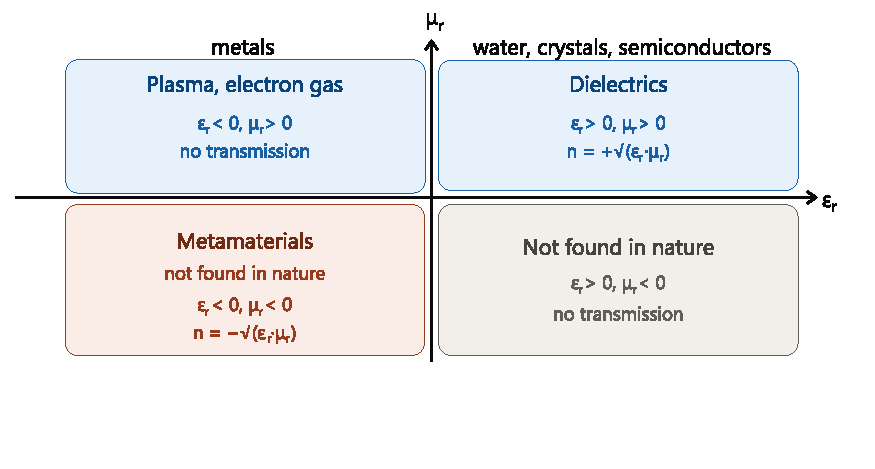
\includegraphics[width=0.68\linewidth]{graphics/materials_classification_epsilon_mu.pdf}
        \caption{Classification of Materials Based on Their Dielectric and Magnetic Properties.}
        \label{fig:materials-classification}
    \end{figure}

        \paragraph{Solution to the wave equation}

        The wave equation is solved by a plane wave of the form

        \begin{equation*}
            \vec{E}(\vec{r},t) = \vec{E}_{0}\,e^{i \, \overbrace{ \left(\vec{k}\cdot\vec{r} - \omega t + \phi\right)}^{\psi} }=\vec{E}_{0}\,\left( \cos(\psi) + i\,\sin(\psi) \right),
        \end{equation*}

        with the physical field understood as the real part, using $e^{i\alpha} = \cos{\alpha} + i\sin{\alpha}$. Here $\vec{k}$ points along the direction of travel, and for this transverse wave the constant vector $\vec{E}_{0}$ is perpendicular to $\vec{k}$. The magnetic field $\vec{B}$ is perpendicular to both, with $|\vec{B}| = \nicefrac{n\,|\vec{E}|}{c}$. The direction in which $\vec{E}_{0}$ points is called the \emph{polarisation} of the wave, discussed next.

    \subsection{Polarisation of a wave}

        Polarisation describes the pattern that the electric-field vector traces out, in the plane perpendicular to the direction of propagation, as the wave passes. Only transverse waves can be polarised. Take propagation along $z$, so that the field lies in the $x$--$y$:

        \begin{equation*}
            \vec{E}(z,t) = \mathrm{Re}\left\{
            \begin{bmatrix}
                E_{x} \\ E_{y}
            \end{bmatrix}
            e^{i(kz-\omega t)}\right\},
        \end{equation*}

        where $E_{x}$ and $E_{y}$ are complex. That pair of complex amplitudes is the \emph{Jones vector}, and it fixes the polarisation completely through their relative size and relative phase. Three cases matter:

        \begin{itemize}
            \item \textbf{Linear} --- the two components are in phase, so $\vec{E}$ stays along a fixed line. Along $x$ the Jones vector is $\left[\begin{smallmatrix}1\\0\end{smallmatrix}\right]$, and at $45^{\circ}$ to the axes it is $\nicefrac{1}{\sqrt{2}}\left[\begin{smallmatrix}1\\1\end{smallmatrix}\right]$. Both entries are real, and a real Jones vector always means linear polarisation.
            \item \textbf{Circular} --- the components have equal size but are a quarter of a period out of phase, so the tip of $\vec{E}$ traces a circle. The Jones vector is $\nicefrac{1}{\sqrt{2}}\left[\begin{smallmatrix}1\\ \pm i\end{smallmatrix}\right]$, and the factor $\pm i$ \emph{is} that quarter-period shift. Taking the upper sign at $z=0$, the real parts are $E_{x} \propto \cos{\omega t}$ and $E_{y} \propto \mathrm{Re}\{ie^{-i\omega t}\} = \sin{\omega t}$: the length of $\vec{E}$ never changes and the vector simply rotates. The sign of $i$ fixes the sense of rotation, and the two are called left- and right-handed, though which is which depends on the convention being used.
            \item \textbf{Elliptical} --- the general case, with unequal amplitudes or any other phase difference, tracing an ellipse. Linear and circular are its two limits.
        \end{itemize}

        The imaginary part is therefore distinguishes a rotating field from an oscillating one.

    \subsection{The laws of reflection and refraction of electromagnetic waves}

        A \emph{ray} is a line drawn along the direction in which the wave (and its energy) travels\footnote{
            True in isotropic media. In birefringent media, energy flow is determined by the Poynting vector and $\vec{k}$ is not points in another direction. Rays naturally are determined by energy flow rather than wavefront orientation.
        }, at right angles to the wavefronts. The laws below are stated in terms of rays.

        \paragraph{The law of reflection}

        The angle of reflection equals the angle of incidence, and the incident ray, the reflected ray and the normal to the surface lie in one plane---\emph{plane of incidence}, which contains the incident ray and the normal. Reflection changes only the direction of propagation, not the wavelength.

        \paragraph{The law of refraction (Snell's law)}

        The incident and refracted rays and the normal lie in one plane, and the angles satisfy

        \begin{equation}\label{eq:snell}
            n_1 \sin \theta_1 = n_2 \sin \theta_2,
        \end{equation}

        where $n_1$, $n_2$ are the refractive indices of the two media (\cref{eq:refractive-index}), $\theta_1$ the angle of incidence and $\theta_2$ the angle of refraction, both measured from the normal.

        A wave is called $p$-polarised (parallel) when its electric field lies in the plane of incidence, and $s$-polarised (perpendicular, from the German \emph{senkrecht}) when its field is perpendicular to it. The fractions of amplitude reflected and transmitted differ for the two, and are given by the Fresnel coefficients.

        \paragraph{The Brewster angle}

        The Brewster angle $\alpha_{B}$ is the angle of incidence at which the reflected and refracted rays are perpendicular to one another. At this angle the reflected $p$-component vanishes, so the reflected light is completely $s$-polarised. It is given by

        \begin{equation}\label{eq:brewster}
            \tan{\alpha_{B}} = \frac{n_{2}}{n_{1}},
        \end{equation}

        with the light incident from the side of medium $n_1$ (taking $n_1 < n_2$). This is how polarising sunglasses work, since light reflected from a road or a water surface arrives close to this angle and is largely polarised in one direction.

        The impossibility of reflectin in-plane $p$-polarisation at the Brewster angle is a consequence of the fact that an oscillating dipole does not radiate along its axis.

    \subsection{The Doppler effect}

        The \emph{Doppler effect} is the difference between the frequency a source emits and the frequency an observer records when the two move relative to one another. For waves that travel in a medium (such as sound) the speeds of source and observer are measured relative to that medium, and the two cases are \emph{not symmetric}. For light in vacuum, which needs no medium, only the relative velocity matters.

        \paragraph{Acoustic (mechanical) waves}

        With $v$ the wave speed in the medium and $v_o$ the observer's speed, $v_s$ the source's speed (both relative to the medium projected onto the path that joins them),

        \begin{equation}\label{eq:doppler-acoustic}
            f' = f\,\frac{v \pm v_o}{v \mp v_s},
        \end{equation}

        where the upper signs apply when that party moves \emph{towards} the other (raising the pitch) and the lower signs when it moves away. Observer and source enter differently: the observer changes the wave speed it meets, while the source changes the wavelength it emits.

        Note the asymmetry between the two limits,
        \begin{equation}
            \left.
            \begin{aligned}
                v_s &\to v      \\
                v_o &\to \infty
            \end{aligned}
            \right\}
            \quad\Longrightarrow\quad
            f' \to \infty,
        \end{equation}
        the source's limit is reached at a finite, physical speed---the wave speed itself--- while the observer's is not, since $v_o$ can grow without bound. Source's speed affect the \emph{weffective avelength}, while the observer's speed affect the \emph{perceived frequency}.

        \paragraph{Electromagnetic waves}

        Here the effect is relativistic and depends only on the relative speed through $\beta = \nicefrac{v}{c}$ (\cref{eq:gamma}). Writing $\phi$ for the angle between the relative velocity and the line of sight,

        \begin{equation}\label{eq:doppler-em}
            f' = f\,\frac{\sqrt{1-\beta^{2}}}{1 \pm \beta\cos{\phi}},
        \end{equation}

        with the upper sign when the two are separating and the lower when they are approaching, exactly as in \cref{eq:doppler-acoustic}. Moving straight along the line of sight ($\phi = 0$) gives the longitudinal case,

        \begin{equation*}
            f' = f\,\sqrt{\frac{1\mp\beta}{1\pm\beta}},
        \end{equation*}

        a redshift when separating and a blueshift when approaching. At $\phi = \nicefrac{\pi}{2}$ the sign stops mattering and what remains is the \emph{transverse} Doppler effect, $f' = f\sqrt{1-\beta^{2}} = \nicefrac{f}{\gamma}$, a pure redshift caused by time dilation that has no counterpart for mechanical waves.

\section{Mechanical waves, electromagnetic waves and de Broglie waves; similarities and differences}
\label{sec:wave-types}

    \begin{itemize}
        \item \textbf{Electromagnetic waves} are oscillating electric and magnetic fields that satisfy the wave equation derived earlier (\cref{eq:em-wave}). They are transverse, travel at $c$ in vacuum and need no medium. In the quantum picture the wave is a stream of photons, each with energy $E = \hbar\omega$ and momentum $p = \hbar k$, where $\omega$ is the angular frequency and $k = \nicefrac{2\pi}{\lambda}$ the wave number.
        \item \textbf{Mechanical waves} are disturbances passing through an elastic medium, as described in \cref{sec:mechanical-media}. They require a medium and may be longitudinal or transverse, with a speed set by the properties of the medium.
        \item \textbf{Matter waves}, or de Broglie waves, express the fact that every particle also behaves as a wave, with the (de Broglie) wavelength
        \begin{empheq}[box=\fbox]{equation}\label{eq:de-broglie}
            \lambda_{\text{dB}} = \frac{h}{p} = \frac{h}{mv},
        \end{empheq}
        \keyeqentry{de Broglie wavelength}
        so the wave nature is easiest to see for light particles such as electrons, whose diffraction and interference are used in electron microscopy and diffraction imaging. A localised particle corresponds not to a single wavelength but to a \emph{wave packet}---a superposition of many waves. 
        
        The same relations $E = \hbar\omega$ and $p = \hbar k$ apply, the second being \cref{eq:de-broglie} written in terms of the wavenumber $k = \nicefrac{2\pi}{\lambda}$. Combining them with the classical $E = \nicefrac{p^{2}}{2m}$ gives the free-particle dispersion relation $\omega = \nicefrac{\hbar k^{2}}{2m}$, so matter waves are \emph{dispersive}---unlike light in vacuum, their speed depends on the wavelength. The packet as a whole travels at the group velocity $\nicefrac{d\omega}{dk} = \nicefrac{p}{m} = v$, recovering the classical particle speed. The phase velocity $\nicefrac{\omega}{k} = \nicefrac{v}{2}$ carries no such meaning, as it describes the motion of the individual crests rather than of the particle.\todoper{Look at QMI}
    \end{itemize}

    \paragraph{Common features and differences}

    All three show interference and diffraction, obey the laws of reflection and refraction, and can form standing waves by superposition. 
    
    They differ in what they need and what they are: mechanical waves need a medium, whereas electromagnetic and matter waves do not. Electromagnetic and matter waves are quantum in nature (although EM waves have a potent classical description)---for a matter wave the squared amplitude gives the probability of finding the particle (\cref{post:born}), while for light it corresponds to the number of photons.

\section{Phase transitions; types of phase transitions, order parameter of phase transition, coexistence of phases (examples of phenomena)}
\label{sec:phase-transitions}

    A \emph{phase} is a region of matter that is uniform in its physical and chemical properties---ice, liquid water and steam are three phases of the same substance. A \emph{phase transition} is a change from one phase to another when a control variable such as temperature or pressure is varied. It may involve the state of matter, the crystal structure or the magnetic ordering.

    \subsection{Which phase is stable}

        At fixed temperature and pressure a system settles at the minimum of its Gibbs free energy $G$ (\cref{sec:thermo-potentials}), so of two candidate phases the stable one is whichever has the lower $G$. For a single substance $G$ is proportional to the amount of material, $G = \mu N$, so the \emph{chemical potential} $\mu = \nicefrac{G}{N}$ is the Gibbs free energy per particle. Using $\mu$ rather than $G$ is what makes the comparison possible at all: $\mu$ is intensive, a function of $T$ and $p$ alone, so it characterises a phase without reference to how much of that phase there is.

        The stable phase is therefore the one of lower $\mu$, and this also fixes what happens at the boundary between two of them. Particles move from high $\mu$ to low $\mu$ in the same way that heat flows from high to low temperature (\cref{sec:thermo-potentials}), so a liquid evaporates for as long as the vapour offers a lower $\mu$ and stops when the two are equal. Two phases coexist in equilibrium exactly when

        \begin{equation}\label{eq:coexistence}
            \mu_1(T,p) = \mu_2(T,p).
        \end{equation}

    \subsection{Types of phase transition}

        Because \cref{eq:coexistence} holds at the transition, $\mu$ itself is continuous there---the phases are equally stable, which is why either can be converted into the other at no cost in free energy. The transition can therefore only announce itself in the \emph{derivatives} of $\mu$, and the \emph{Ehrenfest classification} calls a transition $n$-th order when the $n$-th derivative with respect to $T$ or to $p$ is the first that is discontinuous.

        Those derivatives are not abstract. Writing $G = U - TS + pV$ per particle gives $d\mu = -s\,dT + v\,dp$, so $\left(\nicefrac{\partial\mu}{\partial T}\right)_p = -s$ and $\left(\nicefrac{\partial\mu}{\partial p}\right)_T = v$, the entropy and the volume per particle. The classification is then a statement about measurable quantities.

        \begin{itemize}
            \item \textbf{First order} --- $s$ and $v$ jump. The jump in entropy is heat absorbed at constant temperature, the \emph{latent heat} $L = T\,\Delta s$, and the jump in $v$ is the sudden change of density. Melting and boiling are the examples: water at \qty{100}{\celsius} takes up its latent heat of vaporisation without getting any hotter, and expands by a factor of about $1600$.
            \item \textbf{Second order} --- $s$ and $v$ are continuous, so there is neither latent heat nor a density jump, but a second derivative is discontinuous. The second derivatives are the response functions, among them the heat capacity $c_p = -T\left(\nicefrac{\partial^{2}\mu}{\partial T^{2}}\right)_p$, the compressibility and the thermal expansion. A ferromagnet losing its magnetisation at the Curie temperature is the standard example.
            \item Higher orders are not used in practice, and the scheme itself breaks down whenever a derivative \emph{diverges} instead of jumping, as the heat capacity does at the superfluid transition of helium at \qty{2.17}{\kelvin}. Modern usage therefore keeps only two classes: first-order transitions, which have latent heat, and \emph{continuous} transitions, which do not.
        \end{itemize}

    \subsection{The order parameter}
        \todo{is this the best most concise pricutre?}
        Knowing that a transition occurs says nothing about what changes at it. The \emph{order parameter} $\eta$ is the single number that does: it is chosen to vanish in the disordered, more symmetric phase and to be nonzero in the ordered one, so it measures how much of the ordering has set in.

        Its real use is that it allows a theory of the transition with no microscopic model at all. Near a continuous transition $\eta$ is small, so the free energy may be expanded in powers of it, and symmetry decides which powers may appear. When the two signs of $\eta$ describe physically equivalent states only even powers survive, which gives \emph{Landau theory},

        \begin{equation}\label{eq:landau}
            G(T,\eta) = G_0(T) + a_0\,(T - T_c)\,\eta^{2} + b\,\eta^{4}, \qquad a_0,\,b > 0 .
        \end{equation}

        Above $T_c$ the quadratic coefficient is positive and the only minimum sits at $\eta = 0$. Below $T_c$ it turns negative and the minima move out to $\eta = \pm\sqrt{\nicefrac{a_0(T_c - T)}{2b}}$, growing continuously from zero. The system has to choose one of two equally good minima, which is \emph{spontaneous symmetry breaking}: the free energy retains a symmetry that the state does not. The order parameter also labels the transition, since it grows continuously from zero at a continuous transition and jumps straight to a finite value at a first-order one.

        \begin{itemize}
            \item \textbf{Ferromagnet} --- $\eta$ is the magnetisation $M$. Above the Curie temperature ($T_C = \qty{1043}{\kelvin}$ for iron) the moments point every way and average to $M = 0$, which is the paramagnetic phase. Below it they align along a direction the sample selects for itself, and $M$ rises continuously from zero as the temperature falls.
            \item \textbf{Liquid and gas} --- $\eta$ is the density difference $\rho_{\mathrm{l}} - \rho_{\mathrm{g}}$ between the coexisting phases. It is nonzero everywhere along the coexistence curve and closes to zero at the critical point, beyond which there is one fluid and nothing left to tell apart. Crossing the curve at a temperature below the critical one, the density jumps, which is first order, whereas at the critical point the difference vanishes continuously.
            \item \textbf{Superfluid and superconductor} --- $\eta$ is the wave function shared by the particles of the condensate, its squared modulus giving the density of the condensed fraction: zero above the transition temperature, growing below it.
        \end{itemize}

        The picture is not universal. The liquid--gas transition breaks no symmetry---one may pass from liquid to gas by going round the critical point without crossing any boundary---so there the order parameter is a useful choice rather than something symmetry dictates.

    \subsection{Coexistence of phases}

        How many phases can coexist, and how much freedom remains when they do, follows from \cref{eq:coexistence} by counting. With $s$ components distributed over $r$ phases the unknowns are $T$, $p$ and the composition of each phase, which is $s-1$ independent fractions per phase, so $2 + r(s-1)$ in all. Equilibrium demands that every component have the same chemical potential in every phase, which is $s(r-1)$ equations. What is left over is the number of variables still free, the \emph{Gibbs phase rule},

        \begin{equation}\label{eq:gibbs-phase}
            f = s - r + 2 .
        \end{equation}

        It presumes full equilibrium: a common temperature, a common pressure and \cref{eq:coexistence}. For a single substance ($s = 1$):

        \begin{itemize}
            \item $r = 1$, so $f = 2$ --- $T$ and $p$ may be varied independently and a single phase occupies an area of the pressure--temperature diagram.
            \item $r = 2$, so $f = 1$ --- choosing $T$ already fixes $p$, and coexistence is confined to a curve.
            \item $r = 3$, so $f = 0$ --- a single point, the triple point. For water it lies at \qty{273.16}{\kelvin} and \qty{611.657}{\pascal}, and its sharpness is why it served as the fixed point of the Kelvin scale.
        \end{itemize}

    \subsection{Coexistence in practice}

        Take a sealed rigid vessel part-filled with water and heat it slowly. Liquid and vapour coexist, so $f = 1$ and the pressure is not ours to choose: it climbs along the vapour-pressure curve as the temperature climbs. Heat supplied while both phases are present raises no temperature but converts liquid into vapour, which is the latent heat of a first-order transition. 

        The order parameter is on display throughout. Heating the vessel makes the liquid expand and thin while the vapour is compressed denser, so $\rho_{\mathrm{l}} - \rho_{\mathrm{g}}$ shrinks. If the mean density in the vessel happens to be the critical one, the two densities meet at the critical point (\qty{647}{\kelvin} and \qty{22.1}{\mega\pascal} for water), the meniscus between them fades and a single fluid fills the vessel---the order parameter has gone continuously to zero. Just before it disappears the fluid turns milky and scatters light strongly, an effect called \emph{critical opalescence}, because the density fluctuations have grown to the size of the wavelength of light.

        Melting shows the same pattern with the phases exchanged, so a stirred glass of iced water holds \qty{0}{\celsius} until the last of the ice has gone. The magnetic counterpart is a ferromagnet below its Curie temperature at zero field, where the up- and down-magnetised states have equal free energy and coexist as \emph{domains}. Its field--temperature diagram has the same shape as the pressure--temperature diagram of the fluid, with the Curie point in the role of the critical point.

\section{Experimental foundations of quantum mechanics; examples of phenomena that can be explained in quantum mechanics, but not in classical theory}
\label{sec:qm-experimental}

    Quantum mechanics was forced on physics by a handful of experiments that classical theory gets wrong not merely in detail but in kind. The postulates themselves are set out in \cref{sec:postulates}, and the origin of discrete energies in \cref{sec:quantisation}. What follows is the evidence for them.

    \paragraph{Black-body radiation}

    A \emph{black body}---one that absorbs all radiation falling on it---radiates with a spectrum fixed by its temperature alone. Classically the predicted power diverges towards short wavelengths---the \emph{ultraviolet catastrophe}---whereas the measured spectrum peaks and then falls away. In 1900 Planck reproduced it by assuming that a mode of frequency $f$ exchanges energy only in whole quanta $E = hf$, which makes the short-wavelength modes too expensive to excite. The argument is given in full in \cref{sec:thermal-radiation}.

    \paragraph{The photoelectric effect}

    Light falling on a metal ejects electrons. Classically their energy should grow with the intensity of the light. What is measured is that the maximum kinetic energy of the ejected electrons depends only on the \emph{frequency}, while the intensity fixes only the \emph{number} of electrons, and that below a threshold frequency nothing is emitted however bright the light. This follows if the light arrives as quanta of energy $hf$, one photon freeing one electron against the work function $W$, the least energy needed to pull an electron out of the metal,

    \begin{equation*}
        E_\text{kin}^\text{max} = hf - W .
    \end{equation*}

    \paragraph{The Compton effect}

    X-rays scattered from weakly bound electrons come off with a longer wavelength, the shift growing with the scattering angle $\theta$,

    \begin{equation*}
        \Delta\lambda = \frac{h}{m_e c}\left(1 - \cos\theta\right).
    \end{equation*}

    A classical wave would scatter without changing its wavelength, but this result follows at once if the photon is treated as a particle carrying both energy and momentum, so that the collision is an ordinary elastic one and the photon gives up a share of each.

    \paragraph{Atomic spectra}

    Atoms absorb and emit light only at sharp, characteristic frequencies, and the set of frequencies identifies the element. Classical physics allows a continuous range of orbits and so predicts a continuous spectrum, with no sharp lines at all. The lines follow if the atom has only a discrete set of allowed energies and each photon carries exactly the difference between two of them,

    \begin{equation*}
        hf = E_m - E_n .
    \end{equation*}

    That these levels are a property of the atom and not merely of the light is confirmed by the Franck--Hertz experiment, in which electrons driven through a vapour lose energy only in fixed amounts, so the same discreteness appears with no photon involved.

    \paragraph{The stability of the atom}

    Classical physics also cannot hold the atom together: an orbiting electron is an accelerating charge, so it would radiate continuously and spiral into the nucleus in about \qty{e-11}{\second}. Discreteness of the energies does not by itself cure this, since a Bohr orbit is still an accelerating charge, and Bohr had to impose the stability of his orbits as a separate postulate. Quantum mechanics supplies both facts at once. The allowed energies are discrete because the wave function of a bound particle must meet boundary conditions (\cref{sec:quantisation}), and the atom is stable because that set of energies has a lowest member, so the ground state has nothing to decay into. In any stationary state the probability density does not change with time, so there is no oscillating charge to radiate.

    \paragraph{Interference of single particles}

    Coherent light through two slits gives interference fringes, as any wave would. The quantum result is that electrons fired one at a time build up the same pattern, each arriving as a single localised impact at a point that cannot be predicted. The wave function fixes only the probability, and the fringes come from amplitudes rather than probabilities being added, which is worked through in \cref{sec:postulates}. Merely making it possible to tell which slit was used destroys the pattern, and nothing classical behaves in that way.

    \paragraph{Other purely quantum phenomena}

    There are more purely quantum phenomena: \emph{tunnelling} through a barrier the particle has not the energy to cross (\cref{sec:tunnelling}), the \emph{spin} of the electron, whose projection on any axis takes only two values and which splits a beam of silver atoms into two in the Stern--Gerlach experiment (\cref{sec:atoms-fields}), the \emph{exclusion of identical spin-\nicefrac{1}{2} partcles (fermions)} from a common state (Pauli exclusion principle), which is what gives matter its volume and the periodic table its structure (\cref{eq:identical}), and \emph{entanglement}, in which a pair of particles has a state but neither member has one of its own (\cref{post:composite}).

\section{The uncertainty principle; limits of accuracy of measurements}
\label{sec:uncertainty}

    The Heisenberg uncertainty principle states that certain pairs of observables cannot both have a definite value in the same state: the more precisely one is fixed, the less precisely the other can be. This is a property of the quantum state itself, not a shortcoming of our instruments.

    Whether two observables $\hat{A}$ and $\hat{B}$ can be definite together is decided by their \emph{commutator}

    \begin{equation*}
        \comm{\hat{A}}{\hat{B}} = \hat{A}\hat{B} - \hat{B}\hat{A},
    \end{equation*}

    which measures how much the order of the two operations matters. If it vanishes the observables commute and can be measured simultaneously to any accuracy. If it does not, the spreads of the two quantities obey the relation

    \begin{empheq}[box=\fbox]{equation}\label{eq:uncertainty}
        \Delta A\,\Delta B \geq \frac{1}{2}\left| \comm{\hat{A}}{\hat{B}} \right| .
    \end{empheq}

    Here $\Delta A$ is the ordinary standard deviation of the measured values, built from the expectation values of \cref{sec:postulates},

    \begin{equation*}
        \Delta A = \sqrt{\ev{\hat{A}^{2}} - \ev{\hat{A}}^{2}}, \qquad \ev{\hat{A}} = \bra{\Psi}\hat{A}\ket{\Psi},
    \end{equation*}

    that is, the typical distance of a single result from the mean of many. It is zero exactly when the state is an eigenstate of $\hat{A}$, where every run returns the same eigenvalue.

    The most important case is position and momentum. Since $\comm{\hat{x}}{\hat{p}_x} = i\hbar$, the relation gives

    \begin{empheq}[box=\fbox]{equation}\label{eq:heisenberg-xp}
        \Delta x\,\Delta p_x \geq \frac{\hbar}{2},
    \end{empheq}

    saturated (turned into an equality) by a Gaussian wave packet, which is therefore the best-localised state possible in position and momentum at once. The energy--time relation $\Delta E\,\Delta t \geq \nicefrac{\hbar}{2}$ used in \cref{sec:interactions} looks the same but does not follow from \cref{eq:uncertainty}, because time is a parameter labelling the evolution and not an observable with an operator. There $\Delta E$ is still an ordinary spread, of the energy, whereas $\Delta t$ is a characteristic time---the interval over which the state changes appreciably, which for an unstable state is its lifetime $\tau$ (\cref{sec:light-matter}). This is directly observable: a level that survives only for a time $\tau$ has no sharp energy, so the line it emits is not infinitely thin but spread over an energy $\Gamma \simeq \nicefrac{\hbar}{\tau}$, the \emph{natural linewidth}, the irreducible width of a spectral line.

    The trade-off is easiest to see for a wave. A pure sine wave has a single wavelength, so by the de Broglie relation ($p = \hbar k$ with $k = \nicefrac{2\pi}{\lambda}$, \cref{eq:de-broglie}) its momentum is perfectly defined---but it extends over all space, so its position is completely undefined. A sharply localised spike has a definite position, but building it requires adding together waves of every wavelength (thorugh Fourier series), so its momentum is completely undefined. Any real state is a compromise between these extremes.

    This should not be confused with \enquote{Heisenberg's microscope}, the argument that pinning down a particle's position needs light of ever shorter wavelength, whose photons then carry ever larger momentum and so disturb the particle more. That picture is misleading, because it still assumes the particle has a definite position waiting to be measured, which is exactly what the principle denies.

\section{Approximate methods of quantum mechanics; theory of perturbations for eigenvalues of observables, Fermi Golden Rule, Born approximation for scattering amplitudes}
\label{sec:approximate-methods}

    Quantum mechanics rests on differential equations that can be solved analytically only in a few simple cases, and sometimes even writing down the Hamiltonian is hard. For anything more complicated, approximate methods are used.

    \subsection{Stationary perturbation theory}

        Take a Hamiltonian $\hat{H}_{0}$ we can already solve, that of the hydrogen atom say, and make a small change to the system, such as switching on a weak external electric field. Solving the new problem exactly would be as hard as the original one, so the change is treated instead as a \emph{perturbation}, an extra term $\lambda\hat{H}'$. The method is the quantum counterpart of a Taylor expansion in $\lambda$: successive corrections are added, and the smaller the perturbation the fewer are needed, one or two usually being enough.

        The method is \emph{stationary} in the sense that neither $\hat{H}_{0}$ nor $\hat{H}'$ may depend on time. The perturbed system then still has stationary states of definite energy, and the only question is how those energies and states are shifted. A perturbation that switches on or oscillates is a different problem, treated in \cref{subsec:fermi-golden-rule}.

        With $\lambda$ absorbed into $\hat{H}'$, the corrections to the $n$-th unperturbed level $\left(E_n^{(0)}, \psi_n^{(0)}\right)$ are

        \begin{empheq}[box=\fbox]{align}
            E_n^{(1)} &= \bra{\psi_n^{(0)}} \hat{H}' \ket{\psi_n^{(0)}} \label{eq:pt-e1}\\
            \psi_n^{(1)} &= \sum_{m \neq n} \frac{\bra{\psi_m^{(0)}} \hat{H}' \ket{\psi_n^{(0)}}}{E_n^{(0)} - E_m^{(0)}} \psi_m^{(0)} \label{eq:pt-psi1}\\
            E_n^{(2)} &= \sum_{m \neq n} \frac{|\bra{\psi_m^{(0)}} \hat{H}' \ket{\psi_n^{(0)}}|^2}{E_n^{(0)} - E_m^{(0)}} \label{eq:pt-e2}
        \end{empheq}
        \keyeqentry{Stationary perturbation corrections}

        In words, the first-order shift is the average of the perturbation in the unperturbed state, and the state itself mixes in the other unperturbed states, most strongly those nearest in energy. These formulas hold only for a \emph{non-degenerate} level. If two unperturbed levels share an energy the denominators diverge and the expansion fails, and one must instead diagonalise $\hat{H}'$ within the degenerate set of states---\emph{degenerate perturbation theory}, worked through for the Stark effect in \cref{sec:atoms-fields}.

        Nothing in this is special to energy---the same expansion gives the corrections to the eigenvalues of any observable whose operator is slightly changed---but the Hamiltonian is the case that matters in practice.
        \todoper{Look at QMII}

    \subsection{Fermi Golden Rule}\todoper{A little clearer?}
    \label{subsec:fermi-golden-rule}

        When the perturbation does depend on time, the shifts of the levels are no longer the point. A time-dependent perturbation drives \emph{transitions} between the unperturbed states, and the quantity to compute is the rate at which the system hops from one to another. For a perturbation oscillating at a single frequency, $\hat{H}'e^{-i\omega t}$, first-order time-dependent perturbation theory gives \emph{Fermi's golden rule}

        \begin{empheq}[box=\fbox]{equation}\label{eq:fermi-golden-rule}
            \Gamma_{n\rightarrow{}m} \simeq \frac{2\pi}{\hbar} |\bra{\psi_m^{(0)}}\hat{H}'\ket{\psi_n^{(0)}}|^2 \delta\left(E_m^{(0)} - E_n^{(0)} - \hbar\omega\right)
        \end{empheq}
        \keyeqentry{Fermi Golden Rule}

        The delta function enforces energy conservation: the transition happens only if the quantum $\hbar\omega$ supplied by the perturbation matches the gap between the two levels.

        A delta function only means something once it is integrated over, so the rule applies when the final states form a \emph{continuum}, a dense band of levels rather than isolated ones. Summing over them replaces the delta function by the \emph{density of final states} $\rho$, the number of states available per unit energy,

        \begin{equation}\label{eq:fermi-golden-rule-dos}
            \Gamma_{n\rightarrow{}m} \simeq \frac{2\pi}{\hbar} |\bra{\psi_m^{(0)}}\hat{H}'\ket{\psi_n^{(0)}}|^2 \rho\left(E_n^{(0)} + \hbar\omega\right),
        \end{equation}

        which is the form usually quoted and is the easier one to read: the rate is the strength of the coupling squared, multiplied by how many states there are to go to.

        The standard picture is an excited atom sitting in the electromagnetic vacuum. The field supplies the perturbation, the photon modes the atom can emit into supply the continuum, and the rule returns the spontaneous emission rate and hence the lifetime of the level (\cref{sec:interactions}). A genuinely two-level atom driven by a single wave is \emph{not} an example, because with one final state and no continuum the population swings back and forth between the two levels (Rabi oscillations) instead of leaking away at a steady rate. Being a first-order result, the rule also holds only while the initial state is barely depleted.

    \subsection{The Born approximation}

        The last application is the \emph{Born approximation}\footnote{
            Not to be confused with the Born--Oppenheimer approximation, a different approximation by the same Max Born, which separates the slow nuclear motion from the fast electronic motion in a molecule.
        } for scattering. The experiment it describes is the standard one: a steady beam of particles is fired at a fixed target potential $V(r)$, and detectors placed all round count how many come out per second at each angle. The theory has to predict those counts.

        The beam is described by a \emph{plane wave}, a wave of one wavelength travelling in one direction with the same amplitude everywhere. This is the idealisation of a beam whose particles all share one momentum, which by the de Broglie relation (\cref{eq:de-broglie}) means one wavelength. No real beam fills all space, but one that is broad compared with the target behaves like this, and the plane wave has the advantage of being a steady state, so the problem stays time-independent.

        Far from the target the picture is a ripple tank. Straight crests come in, meet the obstacle, and beyond it there are two things: the original straight wave carrying on, since most of the beam misses the target, and circular ripples spreading outwards from the obstacle. In three dimensions those ripples are an outgoing \emph{spherical wave}, and they are what a detector off to one side registers. They are not equally strong in every direction, and the function giving their strength in the direction $(\theta,\varphi)$ is the \emph{scattering amplitude} $f(\theta,\varphi)$. Its squared modulus $|f|^{2}$ is the \emph{differential cross-section}, an effective target area per unit solid angle, and it is the quantity actually measured.

        The approximation itself is one idea. Think of the potential as a cloud of tiny scattering centres. Each is shaken by the wave passing over it and re-radiates a faint wavelet of its own, and what arrives at the detector is the sum of all those wavelets added together with their phases, so the directions of strong scattering are the directions in which they interfere constructively. What makes the exact problem hard is that each centre is shaken not by the original beam but by the beam already disturbed by all the others. The Born approximation cuts this knot by assuming every centre is shaken by the \emph{undisturbed incoming wave}, which amounts to saying the particle scatters once and then leaves. It is therefore good when the potential is weak or the particle fast, so that the target barely disturbs the beam, and it fails for slow particles or strong potentials that hold the particle long enough for it to scatter repeatedly.

        Adding up wavelets with their phases is exactly what a Fourier transform does, and that is the result worth carrying away: to first order the scattering amplitude is the Fourier transform of the potential. The variable it is transformed against is the \emph{momentum transfer} $\hbar(\vec{k} - \vec{k}')$, the change in the particle's wave vector on scattering, which is small for forward scattering and large for backward scattering. This gives the one qualitative rule to remember---small angles are sensitive to the broad shape of the potential and large angles to its fine detail, in the same way that resolving small features needs short wavelengths. It is why scattering experiments are read backwards: measure the angular pattern, transform it, and recover the potential. That is how the charge distribution inside the nucleus was first mapped, by electron scattering.

        For a spherically symmetric potential the angular part of the transform can be carried out, leaving

        \begin{equation}\label{eq:born}
            f(\theta) = -\frac{2m}{\hbar^2 K}\int_0^\infty r'V(r')\sin(Kr')\,dr',
        \end{equation}

        where $K = 2k\sin(\nicefrac{\theta}{2})$ is the size of the momentum transfer and $k$ the wave number. As a check, putting the Coulomb potential into this returns exactly the Rutherford scattering formula.

\section{The Schrödinger equation as the basis for understanding the structure of the atom and of the chemical molecule; the periodic table of the elements, chemical bonds}
\label{sec:atom-molecule}

    \subsection{The atom from the Schrödinger equation}

        The whole of this section comes out of one equation. A state evolves in time by the Schrödinger equation (\cref{eq:tdse}), and the \emph{states of definite energy are the solutions of its time-independent form} (\cref{eq:tise}). What makes it the basis of atomic and molecular structure is that nothing has to be put in by hand: write down the potential, demand that the solution be physically acceptable, and the allowed energies, the quantum numbers and the shapes of the orbitals all come out as the only solutions those conditions permit. The chemistry then follows from how the solutions are filled.

        For one electron bound to a nucleus of charge $Ze$ the potential is the Coulomb attraction

        \begin{equation*}
            V(r) = -\frac{Ze^{2}}{4\pi\varepsilon_{0}r},
        \end{equation*}

        which depends on the distance alone, so the equation separates in spherical coordinates and every solution factorises into a radial and an angular part, $\psi_{nlm}(r,\theta,\varphi) = R_{nl}(r)\,Y_{lm}(\theta,\varphi)$, the $Y_{lm}$ being the \emph{spherical harmonics}, the standard set of wave shapes on the surface of a sphere. Physically acceptable solutions---finite, single-valued, normalisable---exist only for particular integer labels, the \emph{quantum numbers} (\cref{sec:angular-momentum}):

        \begin{itemize}
            \item \textbf{Principal, $n = 1,2,3,\dots$} --- fixes the energy and roughly the size, $E_{n} = -\nicefrac{13.6\,Z^{2}}{n^{2}}$~eV for a one-electron atom, so $13.6$~eV is the energy needed to remove the electron from hydrogen in its ground state.
            \item \textbf{Orbital, $l = 0,\dots,n-1$} --- fixes the magnitude of the orbital angular momentum, $|\vec{L}| = \hbar\sqrt{l(l+1)}$, and hence the shape. Written as a letter rather than a number: s, p, d, f for $l = 0,1,2,3$, and alphabetically g, h and onwards beyond that.
            \item \textbf{Magnetic, $m = -l,\dots,+l$} --- fixes its projection on a chosen axis, $L_{z} = m\hbar$, that is, the orientation.
            \item \textbf{Spin, $m_{s} = \pm\nicefrac{1}{2}$} --- the projection of the electron's own spin, doubling every count above.
        \end{itemize}

        One such solution is an \emph{orbital}: a spatial probability distribution for one electron, usually drawn as the surface enclosing most of that probability. In hydrogen the three spatial labels do one job each. $n$ sets the size, which grows roughly as $n^{2}$ from the Bohr radius $a_{0} \simeq 0.053$~nm in the ground state. $l$ sets the shape---an s orbital ($l=0$) is a sphere, a p orbital ($l=1$) is two lobes either side of a nodal plane, and the d orbitals ($l=2$) are mostly four-lobed. $m$ sets the orientation of that shape, so the three p orbitals are the same pair of lobes pointing along $x$, $y$ and $z$.\footnote{The directed orbitals drawn in chemistry are real combinations of the complex $\pm m$ solutions, which is why they point along axes rather than carrying a definite $L_{z}$.}

        The three spatial labels nest, each one naming a finer division than the last: $n$ alone names a \emph{shell}, $n$ and $l$ together a \emph{subshell}, and all three an individual \emph{orbital}. Since the exclusion principle (\cref{eq:identical}) forbids two electrons the same four labels, one orbital holds two electrons of opposite spin, a subshell holds $2(2l+1)$---two in s, six in p, ten in d, fourteen in f---and a shell holds $2n^{2}$.

        No exact solution exists once there is more than one electron, because each also repels the others, but the labels survive and the ground state is built by filling the levels according to three rules:

        \begin{itemize}
            \item \textbf{Aufbau principle} --- fill from the lowest energy upwards, in order of increasing $n+l$, and for equal $n+l$ in order of increasing $n$. This is why $4$s fills before $3$d.
            \item \textbf{Pauli exclusion principle} --- no two electrons in one atom share all four quantum numbers.
            \item \textbf{Hund's rule} --- within a subshell, electrons occupy separate orbitals with parallel spins before any orbital takes a second electron.
        \end{itemize}

        The result is the \emph{electron configuration}, written for carbon as $1\text{s}^{2}2\text{s}^{2}2\text{p}^{2}$. Only the outermost, \emph{valence} electrons are available for bonding, and they are what the chemistry of the element is made of.

        \paragraph{Corrections to this picture}

            The energies above are the \emph{gross structure}. Smaller effects split each level further, and it is worth keeping their sizes in order. The \emph{fine structure} comes from relativistic corrections and from the electron's magnetic moment sitting in the field produced by its own orbital motion, the \emph{spin--orbit coupling}. It is smaller than the gross structure by a factor of order $\alpha^{2}\simeq5\times10^{-5}$, where $\alpha \simeq \nicefrac{1}{137}$ is the fine-structure constant. The \emph{hyperfine structure} comes from the far weaker \emph{magnetic moment of the nucleus}, which is built out of the spins and the orbital motion of the protons and neutrons and whose scale is therefore the \emph{nuclear magneton} $\nicefrac{e\hbar}{2m_{p}}$, smaller than the Bohr magneton $\muB$ (\cref{sec:atoms-fields}) by the electron-to-proton mass ratio of about $\nicefrac{1}{1836}$.\footnote{Why a single nucleon has the moment it does---about $2.79$ nuclear magnetons for the proton, and $-1.91$ for the electrically neutral neutron---is a question about the quarks inside it, one level further down and not needed here.} The hyperfine splitting is smaller than the fine structure by roughly that same ratio, and in hydrogen it splits the ground state by about $6\times10^{-6}$~eV, the transition responsible for the $21$~cm radio line used to map galaxies.

            An external field splits levels in its turn, into the Zeeman effect for a magnetic field and the Stark effect for an electric one, both of which are worked out in \cref{sec:atoms-fields}.

    \subsection{The periodic table of the elements}

        The \emph{periodic table} (\cref{fig:periodic-table}) arranges all the chemical elements in order of increasing \emph{atomic number} $Z$---the number of protons in the nucleus, which fixes the identity of the element and equals the number of electrons in the neutral atom.
        \begin{figure}[htbp]
            \centering
            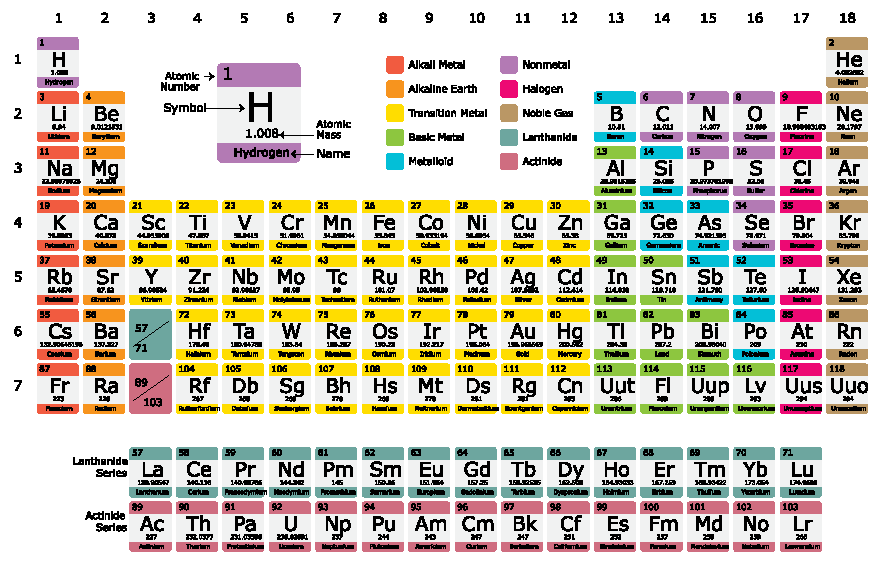
\includegraphics[width=0.9\linewidth]{graphics/periodic-table.pdf}
            \caption{The periodic table of the elements.}
            \label{fig:periodic-table}
        \end{figure}
        The \emph{mass number} $A$, the total number of protons and neutrons, is a separate quantity and is not what orders the table. The modern \emph{periodic law} states that the properties of the elements vary periodically with atomic number. Mendeleev originally ordered the elements by atomic mass, which gives almost the same sequence, but the correct ordering is by atomic number.

        The shape of the table is a direct consequence of the rules above:

        \begin{itemize}
            \item a \textbf{group} (vertical column) collects elements with a similar valence-shell configuration, and hence similar chemical behaviour. The noble gases close a subshell and react with almost nothing.
            \item a \textbf{period} (horizontal row) corresponds to the principal quantum number $n$ of the outermost occupied shell, and its length---$2$, $8$, $8$, $18$---is the capacity of the subshells being filled along it.
        \end{itemize}

    \subsection{Molecules and the different types of chemical bond}

        The same equation applied to two nuclei rather than one explains why atoms stick together. As two atoms approach, each pair of atomic orbitals combines into two \emph{molecular orbitals}: a \emph{bonding} one, in which the two wave functions add and pile electron density up between the nuclei, where it is attracted by both at once and the energy is lowered, and an \emph{antibonding} one, in which they cancel between the nuclei, leaving a node there, and the energy is raised.

        Whether there is a bond is then a matter of counting, since the molecular orbitals form whichever way the electrons are distributed among them. The \emph{bond order} is half the number of electrons in bonding orbitals minus the number in antibonding ones, and it must be positive for the molecule to hold together. Two helium atoms fill the bonding and the antibonding orbital alike, giving bond order zero and no oridinary He$_{2}$ molecule exists.\footnote{
            Helium can only form bonds if it is excited or ionosied or at cryogenic temperatures where the Van der Waals attraction is enough.)
        } Everything below is a special case of valence electrons rearranging in this way to \emph{lower the total energy}.

        \begin{itemize}
            \item \textbf{Ionic} --- one atom transfers electrons to another, and the resulting positive and negative ions attract electrostatically. Both ions are left with closed shells, and a closed shell has a spherically symmetric charge distribution however lopsided its individual orbitals are, so the attraction depends on the separation alone and not on the direction. That is what \emph{non-directional} means here: the structure is fixed by how many ions of one size will pack around another and by overall neutrality, not by any bond angle. The bond is strong, and it forms crystalline solids (e.g.\ NaCl).
            \item \textbf{Covalent} --- neighbouring atoms share pairs of electrons in a common bonding orbital so that each attains a filled valence shell. It is strong and directional, since the orbitals involved are only partly filled and therefore point in particular directions, which is what fixes the shapes of molecules (e.g.\ H$_2$, diamond).
            \item \textbf{Metallic} --- in a metal the atoms are packed so closely that the outermost shell of each overlaps the shells of many neighbours at once. The valence electrons are then not tied to any particular pair of atoms and move freely through the whole solid, leaving positive ion cores in a shared sea of delocalised electrons. Because no bond points anywhere in particular, the ions can slide past one another without the bonding being broken, which is why metals are malleable, and because the electrons are free to move they conduct heat and electricity (e.g.\ copper).
            \item \textbf{Hydrogen bond} --- a much weaker attraction, in which a hydrogen atom already covalently bound to a strongly electronegative atom (O, N, F) is drawn towards a second such atom nearby, the hydrogen being left with little electron density of its own. It holds liquid water together (\cref{fig:water-molecule}) and binds the two strands of DNA.
            \item \textbf{Van der Waals forces} --- the weakest of all, acting between whole neutral molecules with no electron sharing and no charge transfer, and falling off quickly with distance (as $r^{-6}$). They come in three kinds, all dipole--dipole: between two permanent dipoles, between a permanent dipole and the dipole it induces in a neighbour, and between the fluctuating instantaneous dipoles of two atoms whose electron clouds happen to be lopsided at the same moment (the London dispersion force). Only the last is available to a noble gas, and it is what allows even helium to be liquefied. A solid whose lattice points are whole molecules held in place by hydrogen bonds or van der Waals forces alone is called a \emph{molecular} solid---ice and solid carbon dioxide are the standard cases---and such solids are soft and melt at low temperatures. The graphene sheets making up graphite are held to one another in the same way, which is why it flakes so easily.
        \end{itemize}

\section{Quantum tunnelling; examples}
\label{sec:tunnelling}

    \subsection{The barrier problem}

        Quantum tunnelling is the passage of a particle through a potential barrier higher than the particle's own energy---something forbidden in classical mechanics, where the particle simply lacks the energy to get over. The barrier must be finite in both height and width. Against an infinitely high wall the wave function is forced to zero at the boundary and nothing passes, which is why the infinite square well of \cref{sec:quantisation} confines a particle perfectly and the finite well does not.

        Consider a particle of energy $E$ meeting a barrier of height $V_0 > E$ and width $b$. Solving the Schrödinger equation in the three regions gives:

        \begin{itemize}
            \item \textbf{before the barrier} --- an incident plus a reflected wave, $\psi(x) = Ae^{i k x} + Be^{-i k x}$.
            \item \textbf{inside the barrier} --- since $E < V_0$ the wave does not oscillate but decays exponentially, $\psi(x) = Ce^{-\kappa x}$, with $\kappa = \nicefrac{\sqrt{2m(V_0 - E)}}{\hbar}$.
            \item \textbf{beyond the barrier} --- a transmitted wave travelling outwards, $\psi(x) = Fe^{i k x}$, with a smaller amplitude, $|F| < |A|$.
        \end{itemize}

        Because the exponential tail inside the barrier is still nonzero at the far edge, the transmitted amplitude does not vanish: there is a finite probability of the particle emerging. This is measured by the transmission coefficient

        \begin{empheq}[box=\fbox]{equation}
            T = \frac{|F|^2}{|A|^2} \propto e^{-2\kappa b},
        \end{empheq}
        \keyeqentry{Tunneling transmission coefficient}

        the proportionality holding for any barrier thick enough to be worth calling one. Everything about tunnelling follows from that exponential. The probability falls off extremely fast with the width $b$ of the barrier and with $\sqrt{m(V_{0}-E)}$, so tunnelling is a serious effect only for light particles and thin, low barriers, and small changes in any of these quantities change the rate by orders of magnitude.

    \subsection{Examples}

        \begin{itemize}
            \item \textbf{Alpha decay.} An $\alpha$ particle (${}^{4}_2\text{He}^{2+}$) inside a heavy nucleus is held by the strong interaction but faces the Coulomb repulsion of the daughter nucleus as a barrier several MeV higher than its own energy. It escapes by tunnelling. Because $T$ depends exponentially on the energy, a spread of only a few MeV in $\alpha$ energies produces half-lives ranging from microseconds to billions of years, which no other mechanism would explain.
            \item \textbf{Fusion in stars.} Two nuclei must come within about $10^{-15}$~m against their mutual Coulomb repulsion. At the temperature of the Sun's core the typical thermal energy is a thousand times smaller than that barrier, so on classical grounds the Sun should not shine. Fusion proceeds because the rare fast protons tunnel through, and this is also why controlled fusion may be possible at a lower temperature than a classical estimate demands.
            \item \textbf{Scanning tunnelling microscope.} A sharp conducting tip is held a fraction of a nanometre above a surface and a small voltage applied. Electrons tunnel across the gap, and because the current depends exponentially on the width of that gap, moving the tip by the diameter of a single atom changes it by orders of magnitude. Scanning the tip at constant current maps the surface atom by atom.
            \item \textbf{Semiconductor devices.} In a tunnel diode the junction is made so narrow that carriers tunnel straight across it, which gives the device a range of voltages over which the current \emph{falls} as the voltage rises. In flash memory, writing and erasing consist of driving electrons through a thin insulating layer onto an isolated gate, where they stay until driven back.
            \item \textbf{The ammonia molecule.} The nitrogen atom of NH$_3$ sits to one side of the plane of the three hydrogens and tunnels back and forth through it. The two arrangements have the same energy, and the tunnelling splits the ground level into two, the transition between them being the microwave line on which the first maser was built.
        \end{itemize}